% !TeX root = ../main.tex

\chapter{相关工作}

\section{着色器程序优化}

\subsection{GPU 上的实时渲染}

\label{sec:realtime_rendering_in_gpu}

所谓渲染,即是利用计算机程序根据场景中的几何、光照、材质、相机等描述来生成图像的一个过程。根据对真实感的要求以及预期的计算时间开销两个维度,渲染又可以分为离线渲染和实时渲染两大类别。其中,离线渲染往往追求真实的材质、光照表现,而实时渲染则更侧重于画面生成时间的实时性。

% https://en.wikipedia.org/wiki/Geometry_pipelines
% https://www.electronicdesign.com/technologies/embedded/article/21149941/jon-peddie-research-geometry-engine-the-legendary-chip-that-launched-sgi
% https://www.slideshare.net/Mark_Kilgard/sigraph-asia-2008-modern-opengl-presentation#13
% https://dl.acm.org/doi/10.1145/166117.166131 RealityEngine Graphics (SIGGRAPH'93)
% https://www.computer.org/publications/tech-news/chasing-pixels/yamahas-ygy611-a-pioneer-3d-chip
% https://www.computer.org/publications/tech-news/chasing-pixels/1986-ncr-7300 (2d palette only)
% https://www.computer.org/publications/tech-news/chasing-pixels/famous-graphics-chips-hps-artist-graphics
% https://en.wikipedia.org/wiki/Graphics_processing_unit

从算法的角度来看,渲染任务是一个高度并行的计算密集任务,而拥有庞大的分支预测、乱序执行、超标量功能的 CPU 并不天然适合这种任务。在对更高的渲染性能的追求下,适应各种渲染任务或子任务的图形加速器产品应运而生。

早期的图形加速产品通常支持顶点变换、视窗裁剪、透视和正交投影变换,以及直线和样条曲线的生成功能,如 1982 年 SGI 公司的 Geometry Engine \cite{GeometryEngineSGI} 协处理器即为此类产品的范例之一;90 年代中期的产品则多加入着色功能,以支持向多边形图元进行着色,并支持纹理采样、深度缓冲和深度剔除等功能,如 1993 年 SGI 公司的 RealityEngine Graphics \cite{RealityEngineSGI}。图 \ref{fig:reality_engine_graphics} 给出了 RealityEngine Graphics 产品的架构图。可以看到,当时用于交互艺术创作的图形工作站产品已经具有顶点变换、片元生成,以及在片元着色阶段进行纹理采样和多重采样抗锯齿。值得一提的是,这里的“图形流水线”是通过多个 ASIC 拼成的多块板卡实现的,并且可以实现部分的重配置,以适应不同档次的产品所对应的顶点和纹理填充率需求。将绘制流水线中涉及到的多种环节集成到一个 ASIC (专用集成电路)中的 3D 图形处理器,如 1995 年 NVIDIA 公司的 NV1 \cite{NV1NVIDIA, NV1NVIDIANews} 等,则尚不支持硬件加速的顶点变换,而只支持光栅化和后续的着色过程。

随着技术进步和互动娱乐产业的蓬勃发展,图形处理器也逐渐加入了更多功能。例如,2001 年 NVIDIA 公司的 NV20 实现了可编程的顶点变换引擎\cite{10.1145/383259.383274},其可以允许用户在顶点着色阶段传入自定义的着色器程序,而非仅能使用固定管线中有限的功能组合。

截至目前,现在的 GPU 及其对应的 API 接口多支持以图 \ref{fig:rasterize_pipeline} 为基础的光栅化绘制流水线,用于进行 GPU 参与的实时渲染。从图 \ref{fig:rasterize_pipeline} 中可以看到,输入的图元会经历顶点变换、曲面细分、几何着色、光栅化和像素着色阶段,最后在输出合并器 (Output Merger)处将渲染目标(Render Target)送入显存。在这其中,蓝色矩形表示的着色器部分均为可编程着色器部分,可以由程序员经由着色器程序设计语言来编写着色器程序,从而实现自定义的流水线功能。同时,着色器中还可以引用来自显存的其它资源,如纹理、存储缓冲区等 UAV (Unordered Access View)资源。

% \begin{figure}
%     \centering

% \begin{tikzpicture}[node distance=2cm]

% % 定义节点样式
% \tikzstyle{process} = [rectangle, minimum width=4cm, minimum height=1cm, text centered, draw=black]
% \tikzstyle{process2} = [rectangle, minimum width=4cm, minimum height=1cm, text centered, draw=black, rounded corners=.8ex, fill=blue!20]

% % 定义节点
% \node (vertex) [process2] {顶点变换};
% \node (tcs) [process2, below of=vertex] {TCS, 细分着色, TES};
% \node (geometry) [process2, below of=tcs] {几何着色};
% \node (view) [process, below of=geometry] {透视变换};
% \node (clipping) [process, below of=view] {视口裁剪, 背面剔除};
% \node (raster) [process, right = 2cm of clipping] {光栅化};
% \node (earlyZ) [process2, above of=raster] {Early Z, 片段着色};
% \node (zalpha) [process, above of=earlyZ] {深度测试, Alpha混合};
% \node (aa) [process, above of=zalpha] {反走样};
% \node (output) [process, above of=aa] {输出到后端缓冲};

% % 定义箭头
% \draw [->] (vertex) -- (tcs);
% \draw [->] (tcs) -- (geometry);
% \draw [->] (geometry) -- (view);
% \draw [->] (view) -- (clipping);
% \draw [->] (clipping) -- (raster);
% \draw [->] (raster) -- (earlyZ);
% \draw [->] (earlyZ) -- (zalpha);
% \draw [->] (zalpha) -- (aa);
% \draw [->] (aa) -- (output);

% \end{tikzpicture}

%     \caption{光栅化绘制流水线}
%     \label{fig:rasterize_pipeline}
% \end{figure}

\begin{figure}
    \centering
    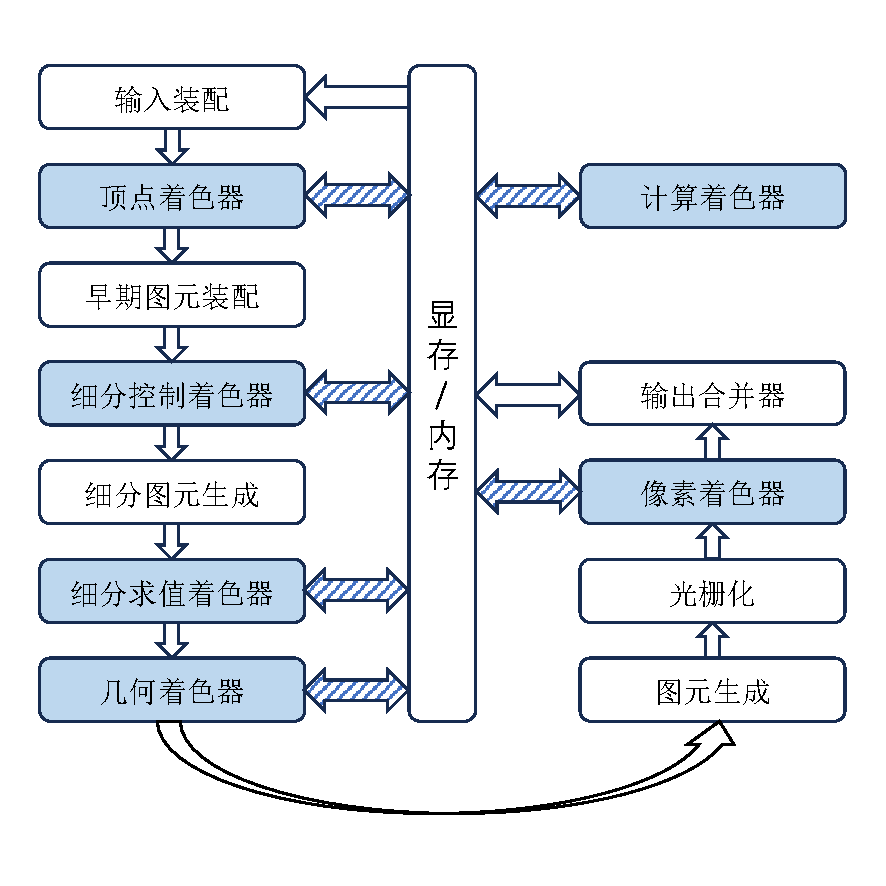
\includegraphics[page=1, width=\linewidth]{figures/pictures.pdf}
    \caption{光栅化绘制流水线}
    \label{fig:rasterize_pipeline}
\end{figure}

% https://gpuopen.com/presentations/2019/nordic-game-2019-triangles-are-precious.pdf
% https://gpuopen.com/wp-content/uploads/2021/01/AMD_Graphics_pipeline_GIC2020.pdf

\begin{figure}
    \centering
    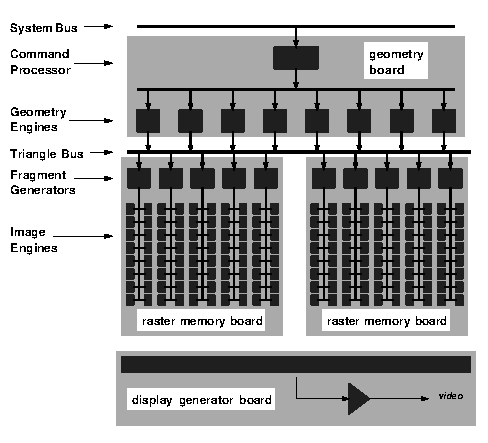
\includegraphics[width=1.0\linewidth]{figures/RealityGraphics-Page2-Crop.pdf}
    \caption{RealityEngine Graphics 架构图\cite{RealityEngineSGI}}
    \label{fig:reality_engine_graphics}
\end{figure}

为了复用顶点着色器和片元着色器阶段中的计算单元以增加算术逻辑运算单元的利用率,从 Xbox 360 \cite{1624324}开始引入了 GPU 统一着色架构(Unified Shader Architecture),并被如 NVIDIA G80 \cite{4523358}后的 GPU 一路沿用。所谓 GPU 的统一着色架构,即包括顶点变换和屏幕空间着色等着色计算在和 GPU 共用的统一的 SIMD 处理器中进行。图 \ref{fig:volta_arch} 为 NVIDIA Volta 架构的示意图,其中包含了对于 GPU 统一计算架构来说比较关键的部分:内存、内存控制器和缓存、SM(Streaming Multiprocessor),线程块调度器和 SM 中的线程束、线程束调度器和计算功能单元。

\begin{figure}
    \centering
    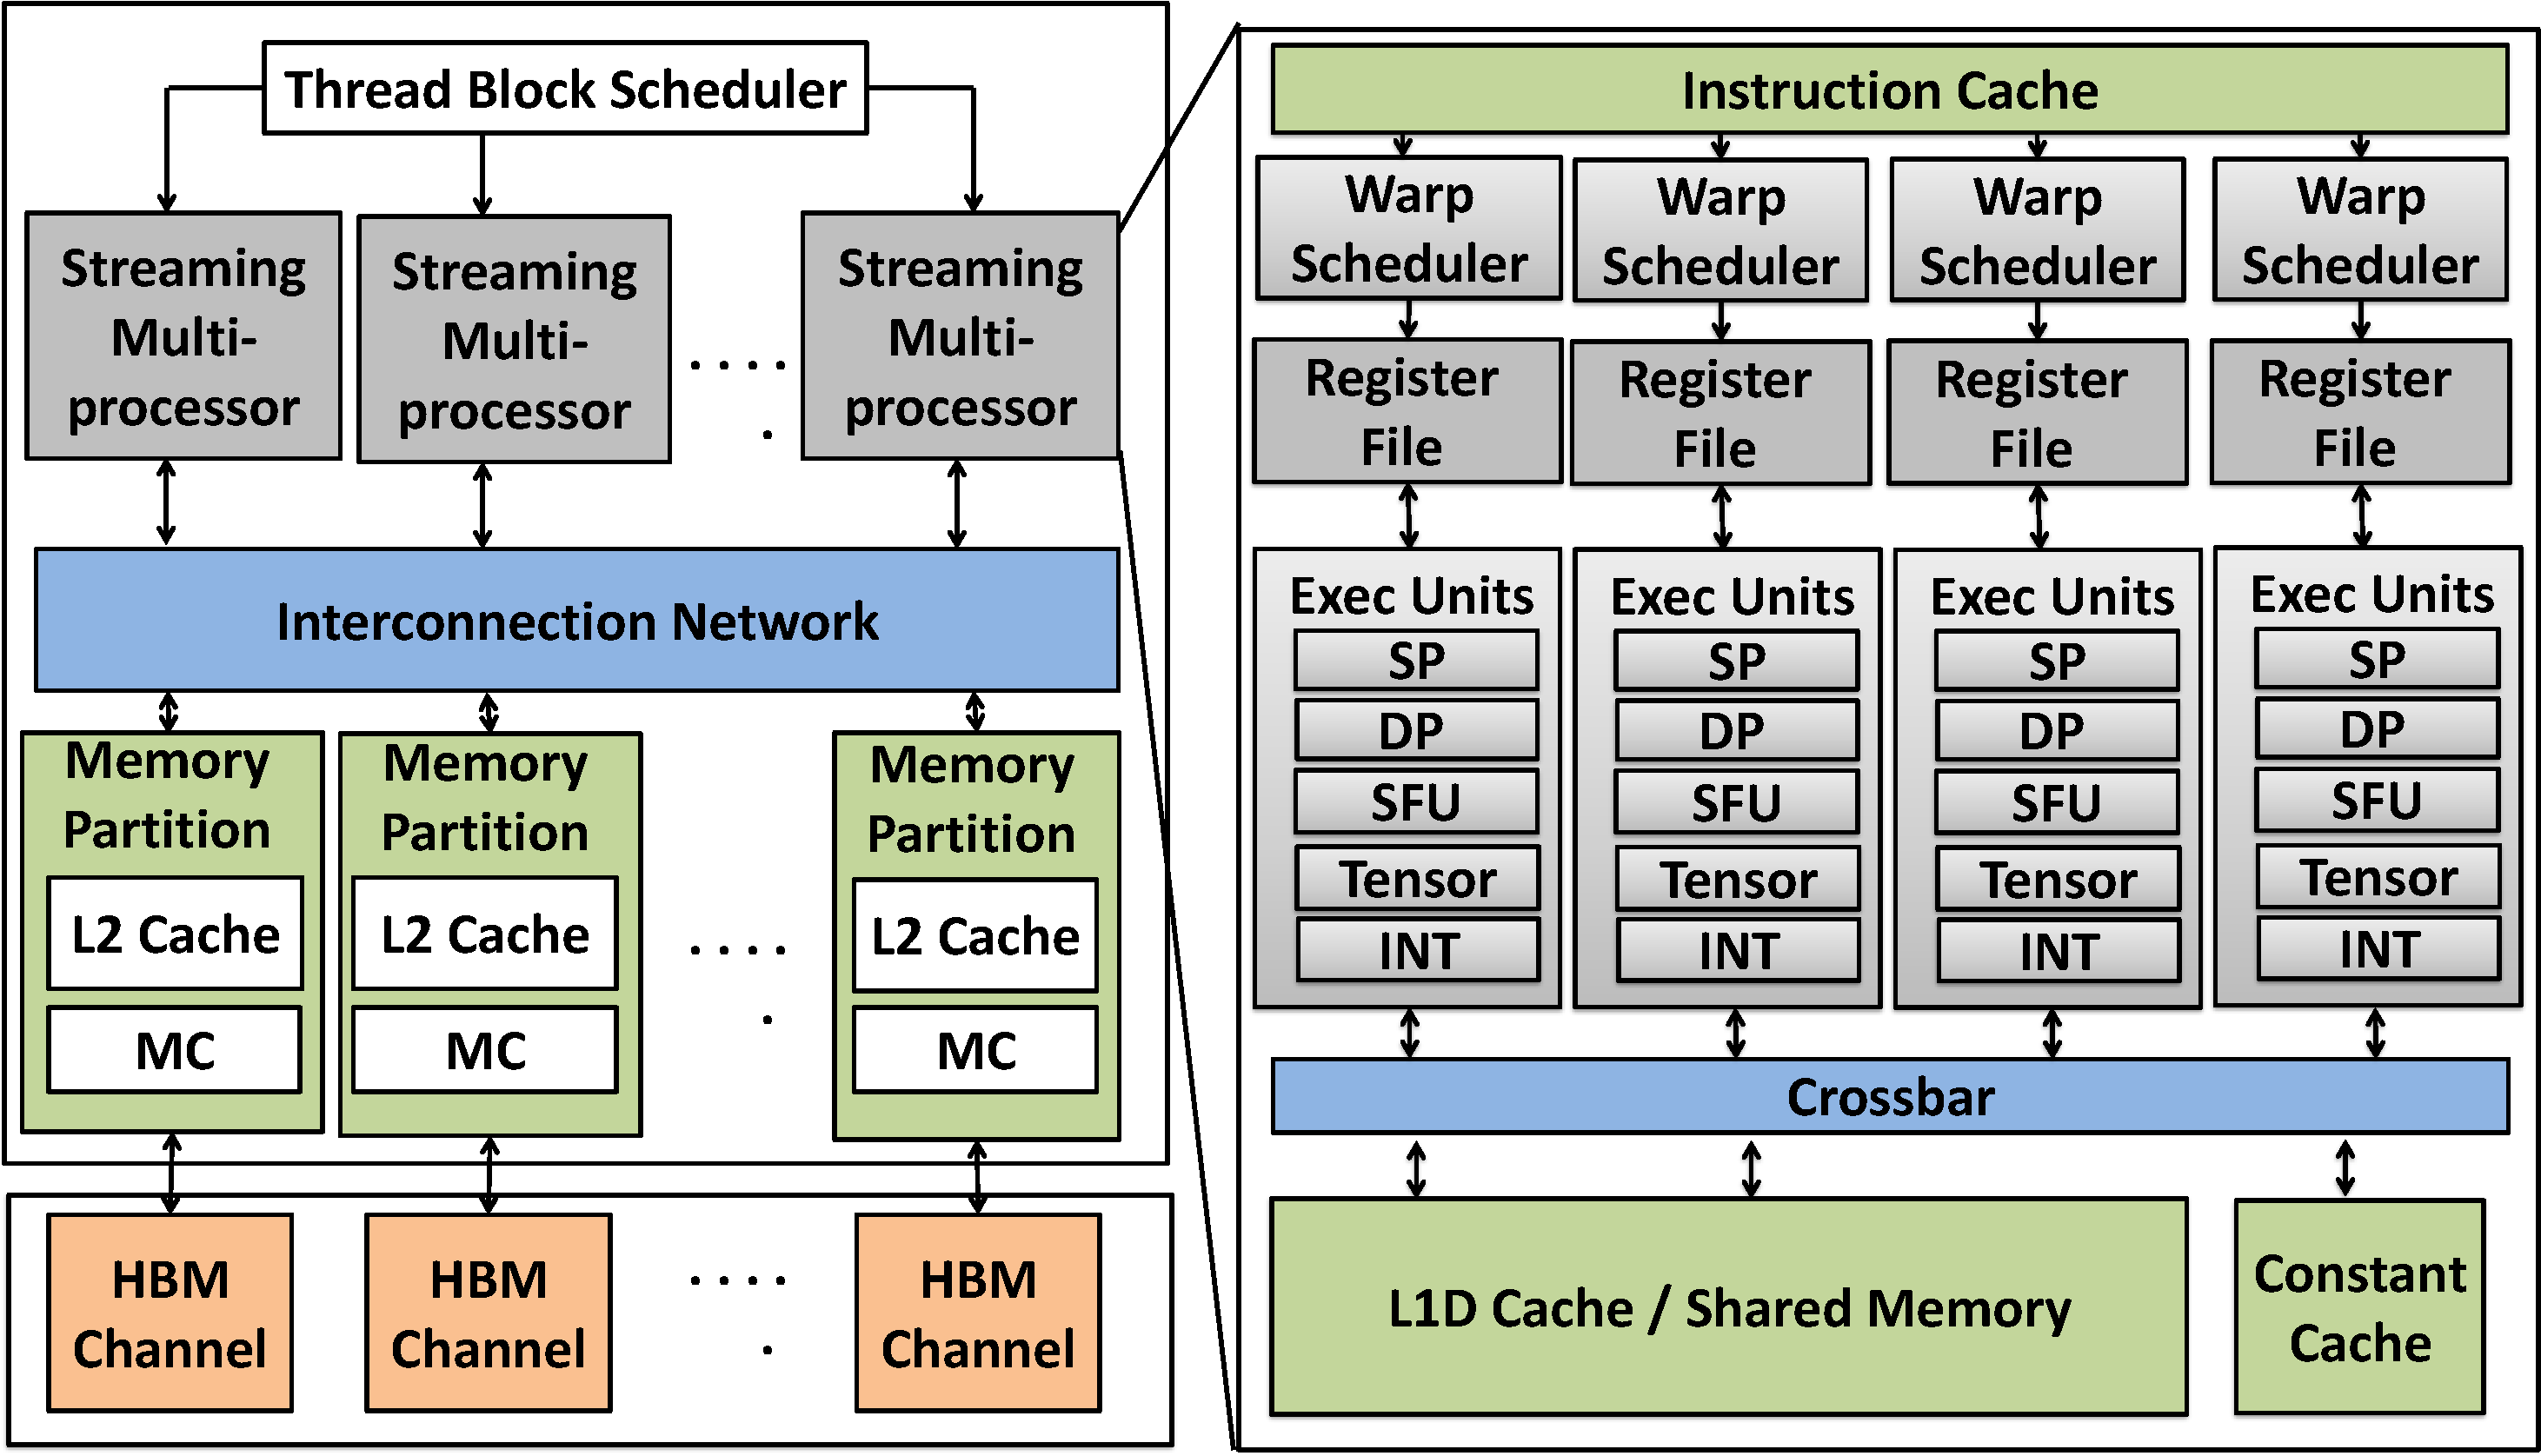
\includegraphics[width=1.0\linewidth]{figures/Volta_archi-crop.pdf}
    \caption{NVIDIA Volta 架构图\cite{9138922}}
    \label{fig:volta_arch}
\end{figure}

用户在编写 CUDA、OpenCL 或者计算着色器(Compute Shader)程序时,对于 GPU 统一计算架构来说比较关键的部分概念会以较为直接的形式映射到用户编写时对应的抽象模型中。譬如,用户编写的描述单个线程行为的程序中,可以用 threadIdx(CUDA)或者 gl\_LocalInvocationID(GLSL 计算着色器)来获得当前线程在抽象的 subgroup 内的索引;再比如,用户可以使用 \_\_shared\_\_(CUDA)或者 shared(GLSL 计算着色器)来定义抽象的 subgroup 内所有线程可以访问的共享内存,这些行为会以比较直接的方式映射到计算架构上,并由具体的调度器进行调度。

然而,对于绘制流水线中的着色过程来说,上述分配则是基本不透明的。同计算着色器或 CUDA 代码一样,顶点、片元和几何着色器程序同样描述了单个“调用”所需要执行的操作;但该调用是如何映射到线程块结构来说是对用户是不透明的,且用户也无法如同计算着色器或 CUDA 核函数那样访问相邻“调用”的局部信息。事实上,这些行为多数是由设备驱动和相关的厂商的硬件实现决定的,并且和架构的实现细节密切相关。

% AMD GPUOpen
% generic informations are not available
% so, want to make step forward

部分厂商会发布面向软件开发者的较为细致的 GPU 编程指南,以供希望了解具体架构的开发者使用。Intel 周期性的发布其显示设备的参考手册,包括 Iris Xe 和 UHD 显示产品,HD 显示产品等\cite{IntelGPUManual},且其内容涵盖 GPU 中多种 IP 核的功能和编程说明、寄存器地址功能参考。AMD 则发布了其 RDNA 架构 GPU 的指令集参考手册\cite{AMDRDNAISA},其中主要描述了其 SIMD 处理器部分的指令参考。嵌入式 GPU 产品厂商也会发布其部分产品的较详细参考手册,如 Broadcom 公司发布的、用于树莓派产品的 VideoCore IV GPU 的架构参考手册\cite{V3DManual}。

然而,如果想要了解给定平台上绘制管线的硬件实现,特别是与性能相关的部分,直接通过上面的手册和材料还是相对困难的。这种困难主要来源于两个方面:其一,并非所有相关的产品细节都会有对应的文档予以发布。例如,对于性能调优有重要意义的 CUDA Binary 为闭源形式,需要进行逆向工程\cite{DecodingCUDABinary};其二,发布的文档中常常含有太多细节,以至于性能相关部分的结构和通路变得较难识别。例如,介绍 Intel Xe 和 UHD 显示核心中渲染引擎(Render Engine)的手册有 723 页,阅读这种体量的文档对于通常对细粒度的绘制流水线的硬件实现不够了解的开发者来说是一种挑战。

本研究提出的方法将着力于通过使用数据驱动的机器学习来对性能进行黑盒建模,以克服利用手册或领域知识进行逐平台的性能分析带来的时间和成本开销上的困难。

\subsection{着色器程序语言}

作为一类领域专用语言(Domain Specific Language,DSL),着色器程序语言是应用在图形 API 中,负责增强和替换图形管线中相应部分固定功能的程序和程序片段编写所用的程序设计语言。

% SEE https://www.nvidia.com/docs/IO/8227/GDC2003_OGL_ARBVertexProgram.pdf and https://www.nvidia.com/docs/IO/8228/GDC2003_OGL_ARBFragmentProgram.pdf

图形程序语言经历了一个从简单到复杂、从低级到高级的过程,这种转变趋势可以从不同的图形 API 中得到证明。2002 年,OpenGL 1.4 引入了 ARB 扩展 ARB\_vertex\_program,其中使用了较为低级的汇编指令形式来描述顶点变换阶段的用户自定义功能。在之后一年的 OpenGL 1.5 中,OpenGL 着色器程序语言 GLSL 的 1.0 版本被引入到 ARB 扩展 ARB\_vertex\_shader 和 ARB\_fragment\_shader 中,并在之后发展迭代,和 OpenGL 标准本身一起演进。

在由 Microsoft 公司主导的 DirectX 图形 API 中,也有类似的发展轨迹。2000 年的 Direct3D 8.0 中,Microsoft 公司引入了使用平台无关的汇编指令来描述顶点变换和像素着色阶段功能的着色器程序模型。之后,在 2002 年的 Direct3D 9.0 中,Microsoft 公司进一步设计了使用高级语言形式来描述顶点变换和像素着色阶段功能的高层次着色语言 HLSL(High Level Shading Language),并且在随后的标准演进中不断增加新功能。

然而,GLSL 和 HLSL 等高层次着色器程序语言因其较为丰富的语法特性,其处理和向 GPU 底层指令的转换均较为复杂。针对这类问题,Khronos Group 提出了一种统一的图形和计算 IR (Intermediate Representation,中间表示),并将其命名为 SPIR-V。经过多年的投入,SPIR-V 成为了 Vulkan 图形 API 的着色器程序输入格式,并且围绕 SPIR-V 有丰富的编译器设施。图 \ref{fig:spirv_ecosystem} 展示了这些编译设施和相应的语言概念,其中语言或指令序列以矩形展示,编译器以圆角矩形展示。

同时,从图 \ref{fig:spirv_ecosystem} 中可以看到,图形程序常用的着色器 GLSL 和 HLSL 可以分别通过 glslang 和 DXC 软件编译到 SPIR-V,进而被实现了 Vulkan 的厂商用户态驱动编译到 GPU 原生指令序列。这套链路相较 OpenGL 中将 GLSL 输入厂商用户态前端来说,因厂商间对 GLSL 语法的一些边缘情况处理不同,故而此套链路在厂商间的一致性会更好。图中的 SPIRV-Cross 软件可以实现 SPIR-V 到 GLSL 和 HLSL 的转译,与前面的前端工具配合的话,可以实现不同着色器语言的互相转换。而图中的 SPIRV-Tools 则可以实现 SPIR-V 中间表示的优化、变换、编排等操作。

% TODO introduce SPIR-V
\begin{figure}
    \centering
    \includegraphics[page=3, width=0.8\linewidth, trim=50 50 50 50, clip]{figures/pictures.pdf}
    \caption{SPIR-V 生态系统}
    % \note{注:语言或指令序列以矩形展示,编译器以圆角矩形展示。}
    \label{fig:spirv_ecosystem}
\end{figure}

本研究的主要目标为构造一个可以适用于各个平台的着色器性能预测器,这样的预测器在着色器语言方面面临着下面两方面的困难:其一,着色器程序可以以多种语言写就,如上文提到的 GLSL,HLSL,Slang,或游戏引擎等采用的更上层的中间格式,且每种格式都有一定的市场占比,没有着色器语言占有绝对的统治地位,而全部支持需要显著的开发和维护开销;其二,前面提到的高层次着色器程序语言往往拥有复杂的语法,不便于进一步的解析和处理。

故而,本研究所提出预测器基于 SPIR-V 中间表示。这样的技术选型正好可以克服上文提到的两个问题:首先,SPIR-V 拥有成熟的转译器(transpiler)生态,GLSL、HLSL 和新型的着色器程序语言 Slang 等均拥有向 SPIR-V 进行转译的工具;其次,SPIR-V 技术设计上即方便进行编译器的编写和编译变换,其采用线性 IR 指令表示,并有简洁清晰的语言规范,成熟可靠的语言优化器等,对本研究后面提及的指令追踪阶段所需要的指令编排工作有一定的帮助。

\subsection{着色器程序优化和简化}

图形 API 本身为了兼容各种不同厂商和架构的底层 GPU 硬件实现,其所希望用户程序本身呈递的着色器程序是贴近高级语言语义的、基本未经历过设备相关的优化、也没有附加很多设备相关语义的着色器程序源语言文本或中间表示。然而,出于图形程序的性能考虑,图形程序员和 GPU 设备厂商通常希望对着色器程序进行一定意义上的优化,使得其在不同或特定平台能拥有较好的实时性能。这样的要求催生了对着色器程序优化和简化的相关工作的探索。

GPU 设备厂商应用的着色器程序优化主要发生在图形程序启动时。此时,图形程序会经由图形 API 向设备驱动呈递着色器程序源码或其中间表示,此时设备驱动中的图形流水线编译器模块将会像传统的 CPU 程序编译器一样,进行源码的中间表示生成,以及编译器后端的设备无关优化、设备相关优化、寄存器分配和指令生成。在这个过程中,编译的速度和编译生成的指令序列的质量都是编译器追求的目标。即便如此,\citet{8366956} 仍然发现设备厂商的驱动并没有充分利用各种可能的着色器程序离线优化机会。\citet{8891638} 也发现,对于输入比较确定的着色器程序,仍然存在进一步优化的空间。

设备驱动中的优化需要基本保证优化后的程序符合原来输入程序的运行结果,但是对于图形应用来说,进行输出完全符合原状的着色器程序优化对于如游戏等应用场景来说并不是必需的。故而,有一系列工作 \cite{10.1145/3528233.3530722, 10.1145/2661229.2661276, 10.1145/2070781.2024186, 10.1145/2816795.2818104, 9815871} 探索了如何在有损条件下,权衡画面表现和运行性能来进行着色器程序简化。这些工作通常使用遗传算法(Genetic Programming,GP)和贪心算法来实现。在遗传算法的每步迭代中,这些工作通常会考虑各种可能对画面造成损失的简化方法:例如,将决定着色器输出的表达式的某个子表达式的值替换为零或该表达式在各种光照条件下的求解结果的平均值,或者将片段着色器阶段进行计算的值移动到顶点着色阶段等。为了进一步加快遗传算法的变异-迭代过程,\citet{10.1145/3528233.3530722} 提出了ShaderTransformer,该方法利用深度学习提出了一个着色器简化变体的渲染质量质量预测器。

\begin{figure}
    \centering
    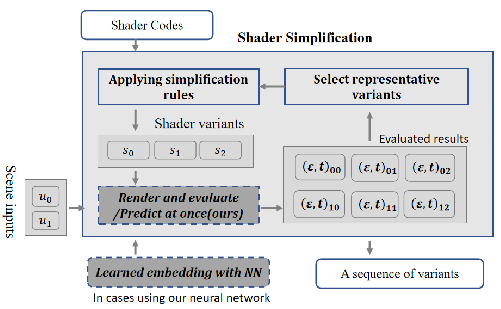
\includegraphics{figures/ShaderTransformer-Pipeline.pdf}
    \caption{ShaderTransformer 使用的着色器简化框架\cite{10.1145/3528233.3530722}}
    \label{fig:shdrTxfmr-framework}
\end{figure}

\begin{figure}
    \centering
    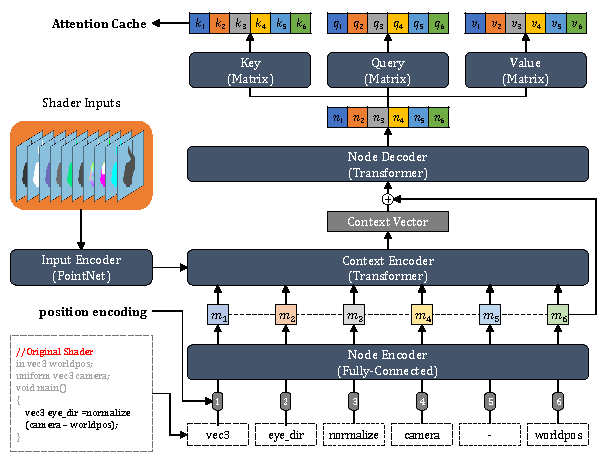
\includegraphics{figures/ShaderTransformer-Flow.pdf}
    \caption{ShaderTransformer 网络架构图\cite{10.1145/3528233.3530722}}
    \label{fig:shdrTxfmr-arch}
\end{figure}

图 \ref{fig:shdrTxfmr-framework} 给出了 \citet{10.1145/3528233.3530722} 的 ShaderTransformer 所使用的着色器程序简化框架。在每轮优化迭代中,着色器程序经过化简会形成一系列的着色器变体 $ s $,而 ShaderTransformer 可以通过 Transformer 来学习并预测每个变体在表示渲染质量中的隐空间的表示,以供评价着色器变体距离简化前的着色器的渲染质量差异 $ \epsilon $。渲染质量差异 $ \epsilon $ 和变体运行时间开销 $ t $ 会为下一步的遗传算法迭代提供参考。

值得注意的是,目前在有损着色器简化的工作通常局限于使用比较简单的启发式算法来表示着色器的运行时开销\cite{10.1145/2816795.2818104, 10.1111/cgf.13482, 10.1145/3528233.3530722},又或者每次评估变异后的着色器程序时进行单独的测量运行\cite{10.1145/2661229.2661276}。对比这些工作,本研究提出的预测器可以在不需要在目标平台上进行单独执行的条件下,对变异后着色器的运行时间开销做出更精确的预测。

图 \ref{fig:shdrTxfmr-arch} 给出了 ShaderTransformer 网络部分的架构图,其中网络的输入包括着色器程序变体的 main 入口函数的函数体源码和着色器程序变体运行时的输入,并通过编码器-解码器架构来得到在渲染质量隐空间中的特征向量。本研究也受到 ShaderTransformer 使用 Transformer 来间接预测着色器变体渲染质量的启发,同样采用 Transformer 网络来预测着色器在目标平台的性能。与其不同的是,ShaderTransformer 使用 PointNet\cite{8099499} 来提取着色器输入信息,而本研究采用了 SPIR-V 中间表示和基于 SPIR-V 的指令追踪技术,从而以统一的方式处理各种类型的输入,同时克服 ShaderTransformer 本身只能处理无分支、单函数的简单片元着色器的缺陷。

\section{程序语言理解}

\label{sec:pl_understanding}

\subsection{语言模型}

\label{sec:language_model}

语言模型是自然语言或程序语言的概率模型。一个语言模型通常定义了语言中文本 $\{l_1, l_2, ..., l_m\}$ 与分词后形成的词元 $\{w_1, ..., w_n\}$ 的对应关系,以及对于句子 $ w_1, ..., w_{i-1} $ 来说,词元 $ w_i$ 出现几率的概率模型 $P(w_i|w_{i-1}, ..., w_{1})
$。

% TODO: add bigram, trigram, ...

对于语言模型来说,将源语言文本转换为词元的分词过程对后续处理有一定影响。对于自然语言文本,各个单词出现的机率并不是均匀的,而对于出现次数过于稀疏的生僻词语,语言模型对其的概率估计总体来说较为困难。为了解决这个问题,BPE(Byte-Pair Encoding)\cite{sennrich-etal-2016-neural} 使用了一种被称为 subword 的单位来进行分词,并被 SentencePiece \cite{kudo-richardson-2018-sentencepiece} 等方法使用。

\subsection{注意力机制与 Transformer 网络}

注意力机制是模仿认知活动中注意力活动的一类神经网络机制。在使用注意力机制的网络中,通常会根据序列内容,为序列中的每个词元生成一个软的权重,并根据部分或全部序列中词元的权重来进行后续的计算。

基于 \citet{bahdanau2016neural} 中注意力机制的工作,\citet{Vaswani2017AttentionIA} 在 2017 年提出了被称为 Transformer 的神经网络结构,在自然语言处理的各类任务上均取得了巨大的成功。Transformer 网络总的结构如图 \ref{fig:transformer_overview} 所示。

\begin{figure}[h]
  \centering
  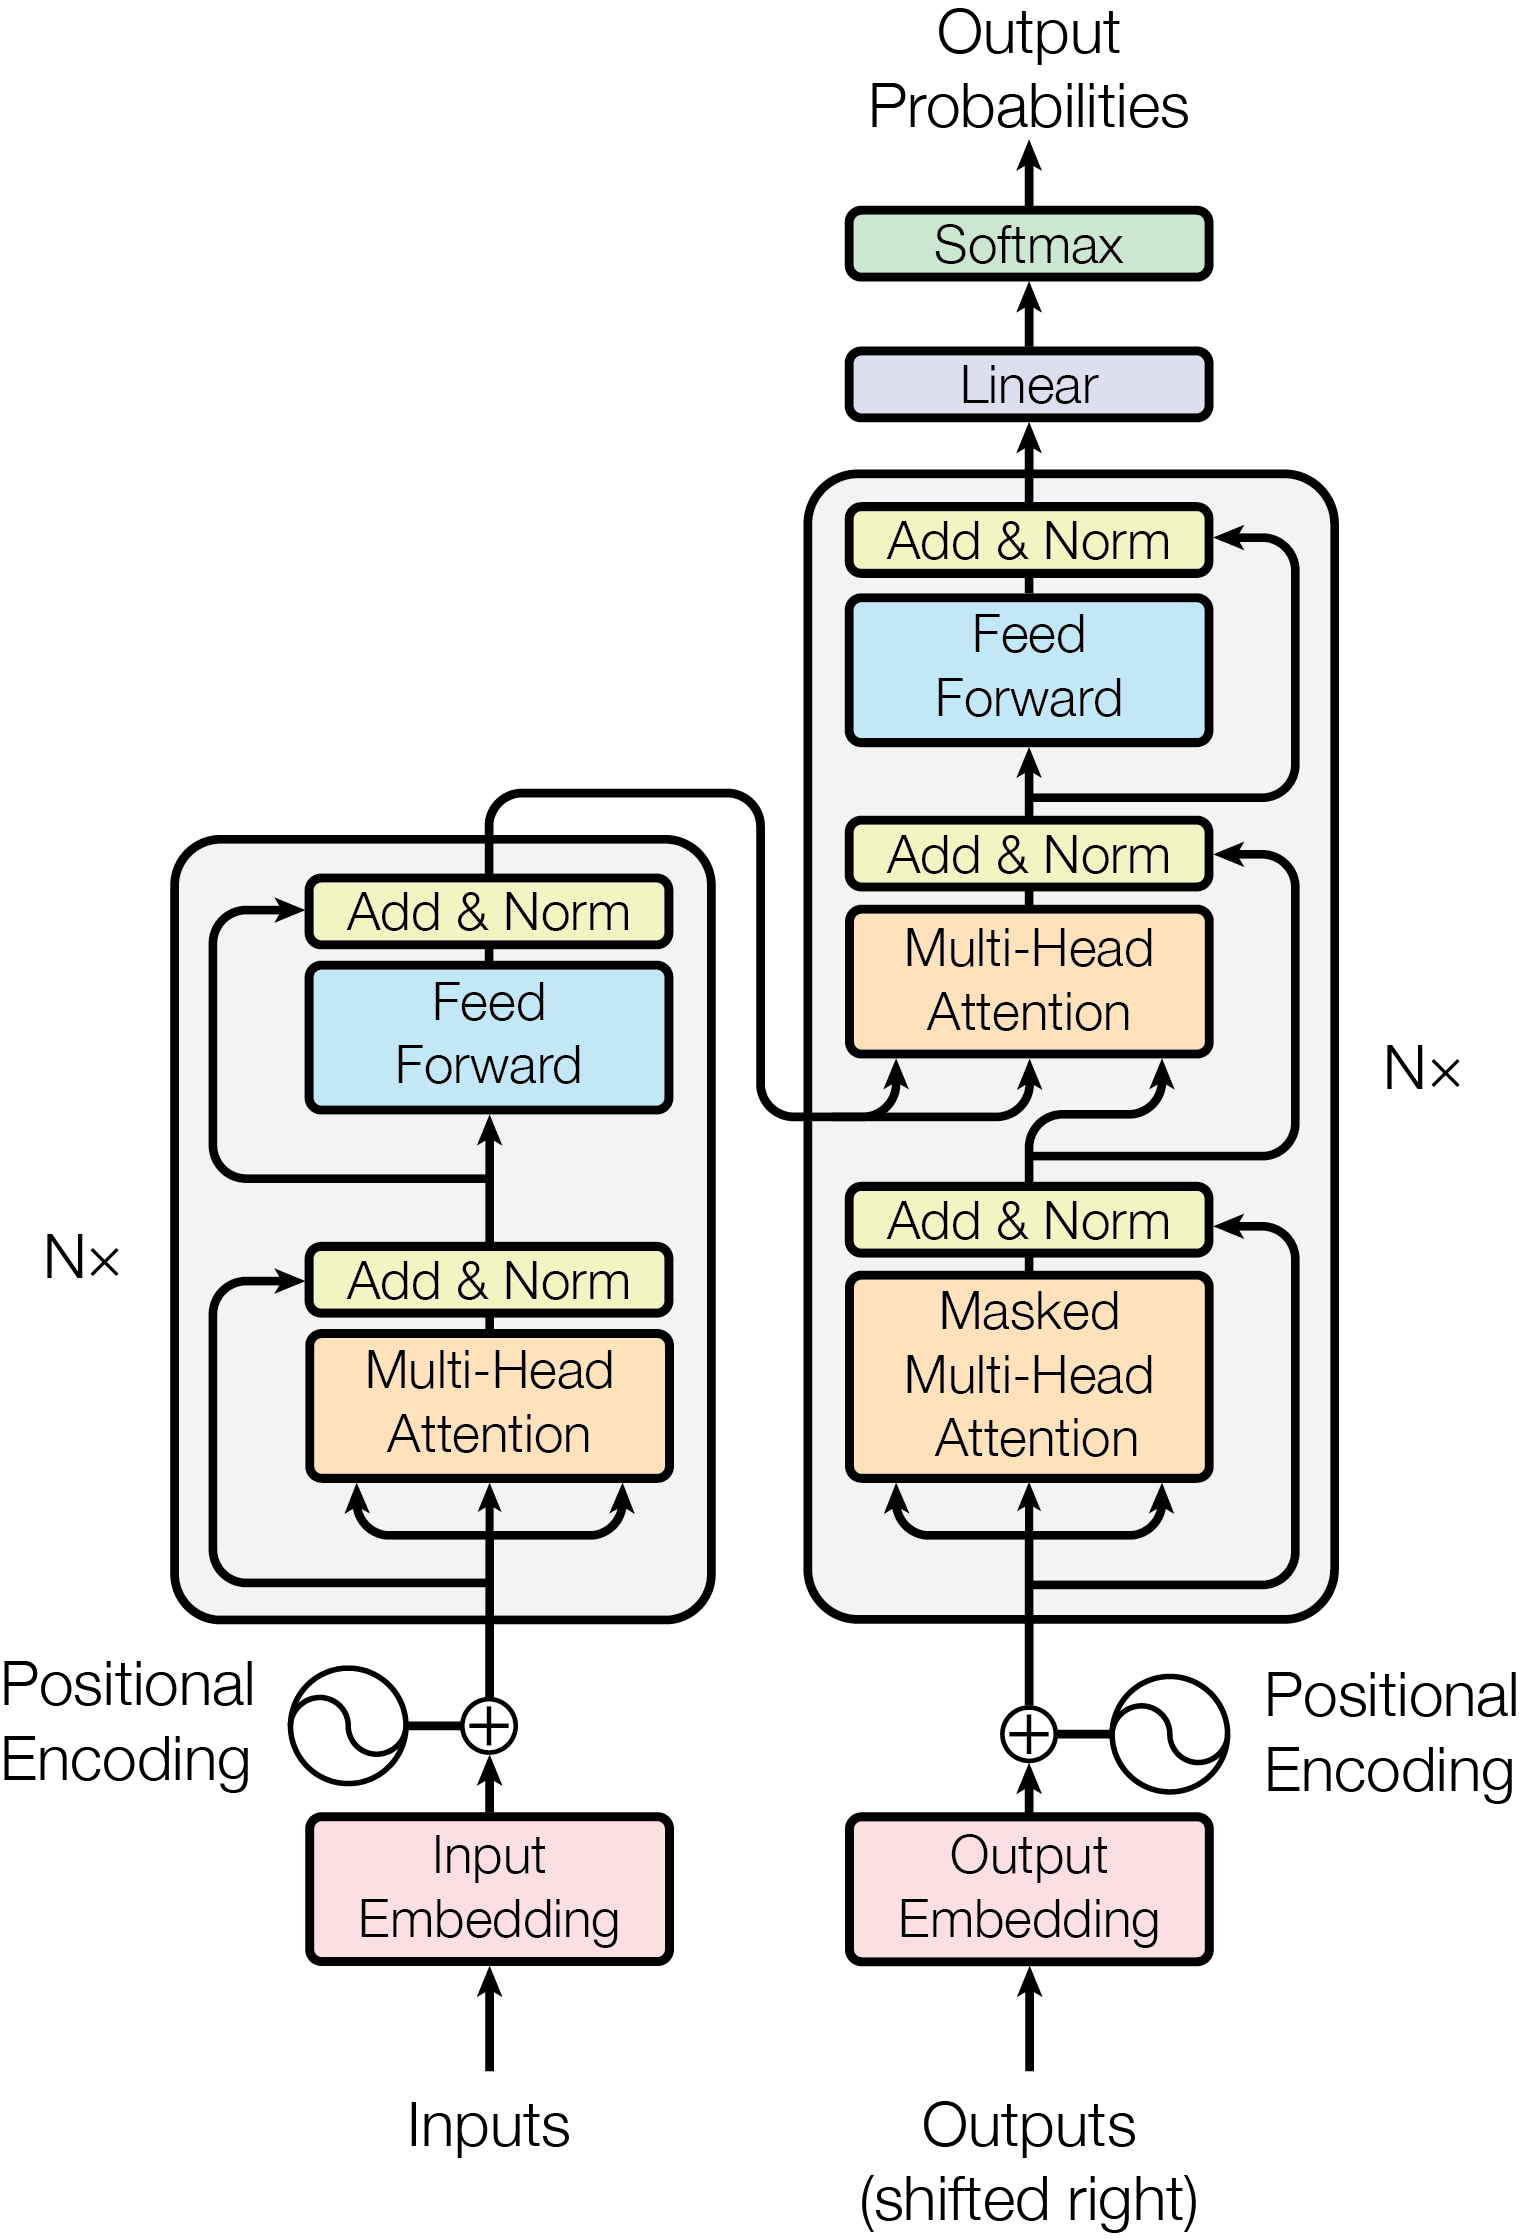
\includegraphics[width=0.5\linewidth]{figures/Transformer-Arch.png}
  \caption{Transformer 网络结构总览\cite{Vaswani2017AttentionIA}}
  % \Description{}
  \label{fig:transformer_overview}
\end{figure}

% generated by gpt3.5; TODO: rewrite

原始版本的 Transformer 模型的网络结构主要由编码器(Encoder)和解码器(Decoder)两个组件构成。Tranformer 的编码器负责将输入的序列转换为相应长度的特征向量,而 Transformer 的解码器则会利用这些特征向量来生成输出序列。

Transformer 的编码器和解码器都由多个相同的基本层堆叠而成,其每个基本层都由两个子层组成:多头自注意力层(Multi-Head Self Attention)和前馈神经网络层(Feed-Forward Neural Network)。这两个子层之间使用层归一化(Layer Normalization)和残差连接(Residual Connection)来连接在一起;同时,在层内的一些位置还会加入 Dropout 层进行归一化。

多头自注意力层由多个相同结构的自注意力层构成。在每个自注意力层中,输入的序列会被分别线性变换到三个被称为查询(Query)、键(Key)和值(Value)的序列。随后,这三个序列会进行一个被称为缩放点积注意力(Scaled dot product attention)的操作
$$
\operatorname{Attention}(Q, K, V) = \operatorname{softmax}\left(\frac{Q K^T}{\sqrt{d_k}}\right)V,
$$
其中 $Q$ 为查询,$K$ 为键,$V$ 为值,$d_k$ 为键的维度。

这种类型的注意力机制可以允许序列中任意的两个位置的词元交换信息,且通过注意力分数来表征了每个位置对其他位置的“重要性”,从而实现了序列中不同位置之间的交互和信息传递。

将维数为词元嵌入维度 $ d_{model} $ 的序列并行的进行多组自注意力操作可以改善模型表现。多个这样的注意力机制进行拼接的结果为多头注意力,其计算方式如下:
$$
\operatorname{MultiHead}(Q, K, V) = \operatorname{Concat}(head_1, ..., head_h) W^{O}
$$
其中 $head_i$ 为第 $ i $ 组独立的进行自注意力计算的计算结果。

多头自注意力层之后,连接的另一个重要模块是前馈神经网络层。该层由两个全连接层组成,并通过 ReLU 函数进行激活,其计算方式如下:
$$
\operatorname{FFN}(x)= \max(0, x W_1 + b_1) W_2 + b_2
$$

原始的 Transformer 中同时使用了编码器和解码器,而编码器和解码器之间还有一个重要的结构:编码器-解码器注意力层(Encoder-Decoder Attention)。在解码器中,每个位置的输出依赖于编码器中所有位置的输入。为了实现这种全局的依赖关系,解码器的多头注意力层中使用了编码器的输出来作为查询 $Q$ 和键 $K$。

总体来看,Transformer 模型通过自注意力机制和多头注意力机制,有效地捕捉了输入序列中的全局依赖关系,并在许多自然语言处理任务中取得了显著的性能提升。例如,BERT \cite{devlin-etal-2019-bert} 模型就利用预训练的范式,在 Transformer 编码器的基础上利用掩码语言建模(Masked Language Modeling)和后续语句预测(Next Sentence Prediction)任务在大规模预料上进行预训练,其在下游任务上只需接受较少的微调即可达到较好的性能。

\subsection{程序设计语言理解任务}

程序设计语言可以被看作一种特殊形式的语言,故而很多自然语言处理领域的方法也适用于程序设计语言的相关任务中。在如 Transformer\cite{Vaswani2017AttentionIA} 和 BERT\cite{devlin-etal-2019-bert} 等模型的影响下,业界涌现出了一批用于程序设计语言任务的模型,如 CodeBERT\cite{feng-etal-2020-codebert},GraphCodeBERT\cite{DBLP:conf/iclr/GuoRLFT0ZDSFTDC21} 等。

\begin{figure}
    \centering
    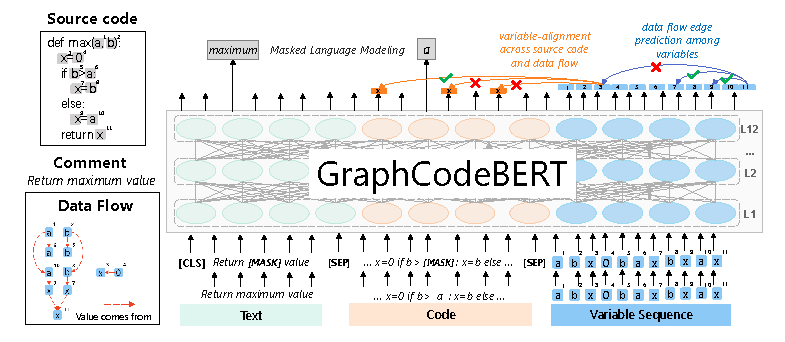
\includegraphics[width=1.0\linewidth]{figures/GraphCodeBERT-Crop.pdf}
    \caption{GraphCodeBERT 架构和预训练示意图\cite{DBLP:conf/iclr/GuoRLFT0ZDSFTDC21}}
    \label{fig:graphCodeBERT_arch_and_pretrain}
\end{figure}

以 GraphCodeBERT 为例,图 \ref{fig:graphCodeBERT_arch_and_pretrain} 给出了 GraphCodeBERT 的架构以及其预训练任务示意图。在模型的训练阶段中,GraphCodeBERT 模型使用了带有注释的源代码和其对应的数据流信息作为输入,并用掩码语言建模和两个和程序语言理解相关的结构化任务来进行预训练。这两个结构化任务分别要预测数据流中的边的起点和终点、以及数据流节点和代码中变量的对应关系。通过模型在大规模程序语料上的预训练工作,特别是程序相关的数据流任务的预训练工作,模型可以提升对于程序设计语言的理解能力,进而提升在如代码搜索、克隆检测等下游任务上的性能表现。

GraphCodeBERT 启发我们,代码的中间表示形式(如抽象语法树)相比源代码文本,能提供更丰富的结构化信息。故而,本研究选择首先将着色器程序编译为中间表示,以作为模型的输入。同时,GraphCodeBERT 等模型采用 Transformer 来程序的变量和指令之间的上下文依赖关系,类似的,本研究的工作也采用 Transformer 来捕捉着色器指令间的上下文相关性,来将更多的上下文信息引入到性能建模中。

根据 \citet{ijcai2022p775} 的综述,程序语言理解模型的典型应用包括抄袭检测,代码分类,代码缺陷检测,代码翻译,代码检索等。同时,也存在被设计为捕捉性能相关的语义的一类任务,譬如在 \citet{8091247} 的工作中引入,并被后续工作 \cite{pmlr-v139-peng21b, pmlr-v139-cummins21a} 用于评价模型质量的 OpenCL 异构架构映射任务。该类任务的输入是一系列 OpenCL 核函数(kernel function),程序语言理解模型需要给出某个具体的核函数在何种平台上运行较快的分类值。笔者希望,通过本研究过程中收集的着色器性能数据,可以启发出更多关于程序语言模型中进行性能语义理解任务的工作。

\section{程序性能建模}

程序性能建模对于计算机软件架构设计和实现中的众多决策都有比较重大的意义,所以学术界开展了大量的、不同计算平台上的,对在 CPU,GPU 和其它加速器上运行的程序进行程序性能估计的工作。这些工作可以依照其建模方法大致分为两种类型的模型:\textbf{基于分析的模型}和\textbf{基于学习的模型}。同时,本章还简要介绍了对于 GPU 上图形系统建模的相关工作。

% Performance modeling is crucial for many design decisions; consequently, extensive research has been dedicated to the estimation of program performance on various computing platforms, including CPU, GPGPU, and other Domain-Specific Architectures (DSAs). Predominantly, the field employs two categories of models: analytical-based models and learning-based models. Works on graphics performance modeling are also discussed in this section. 

\subsection{基于分析的模型}

基于分析的模型可以大致分为\textbf{体系结构模拟器}和\textbf{简单分析模型}两类。

体系结构模拟器是针对性能关键部件进行建模以达到在时钟周期数量级上精确的,人工编写的模拟器。比如,NaviSim \cite{10.1145/3559009.3569666} 是为 AMD RDNA 通用 GPU 架构设计的模拟器,其通过为 wavefront 调度,RDNA 指令发射、解码和执行阶段编写模拟例程来实现计算核函数性能的预测。GPGPU-Sim \cite{9138922, 4919648} 是面向在 NVIDIA GPU 上执行的 CUDA / OpenCL 算例编写的模拟器。

简单分析模型是利用简单的抽象来捕捉其预期描述的架构的公共部分的一类分析模型。这类模型中比较主流的模型有 Roofline 模型\cite{10.1145/1498765.1498785, KONSTANTINIDIS201737}和流水线模型\cite{LEMEIRE202332, 10289219, 10.1145/3524059.3532396}。 

以 Roofline 模型为例,该类模型主要通过利用计算系统中存储器和运算器两个方面的基础数据,来给出待建模系统在稳态条件下的峰值性能估计。

具体来说,Roofline 模型用如下参数刻画给定应用或算例的基本性质:

\begin{itemize}
    \item $W$: 对于给定应用或算例的总计算数目,单位为 FLOP (浮点运算数, FLoating point OPerations)
    \item $Q$: 对于给定应用或算例的总内存访问数,单位为字节
    \item $I = W/Q$: (\textbf{计算强度}, Arithmetic Intensity) 单位内存访问可以完成的计算数目,单位 FLOP/字节
\end{itemize}

此外,定义

\begin{itemize}
    \item $\pi$: 峰值性能,单位为 FLOPS (每秒浮点运算数, FLoating OPeartions per Second)
    \item $\beta$: 峰值存储器带宽,单位为 字节/秒
\end{itemize}

Roofline 模型定义的给定程序的\textbf{可达性能} P 则可以由下式计算:
$$
P = \min(\pi, \beta \cdot I)
$$

从而,可达性能 $ P $ 关于计算强度 $ I $ 的关系又可以用图 \ref{fig:roofline_graph} 来表示。图中曲线即为应用程序在该平台上应用 Roofline 模型计算出来的理论性能峰值,可以看到随着应用程序本身的性质带来的计算强度 $ I $ 的改变,其可达性能可以拥有不同的值。图 \ref{fig:roofline_graph} 中的 I 区域代表由于内存带宽限制了可达性能的访存瓶颈(Memory bound)区,而 II 区域代表由于运算器速率限制了可达性能的计算瓶颈(Compute bound)区。这里假设计算系统参数 $\pi$ = 10 FLOPS,$\beta$ = 1 字节。

值得注意的是,由于指令并行度、发射冲突等架构设计原因,即使理论的内存带宽充足,应用程序对应的指令序列仍可能在使用运算器时遇到无法达到理论的运算器使用率的情形,此时应用程序的性能将低于 Roofline 模型给出的可达性能。同时,由于各种图形处理器中存储器层次结构的存在,不同的存储器层次拥有不同的总带宽,此时有效带宽也将和具体的程序发生耦合,让此类模型的预测变得更加困难。

\begin{figure}[h]
  \centering
  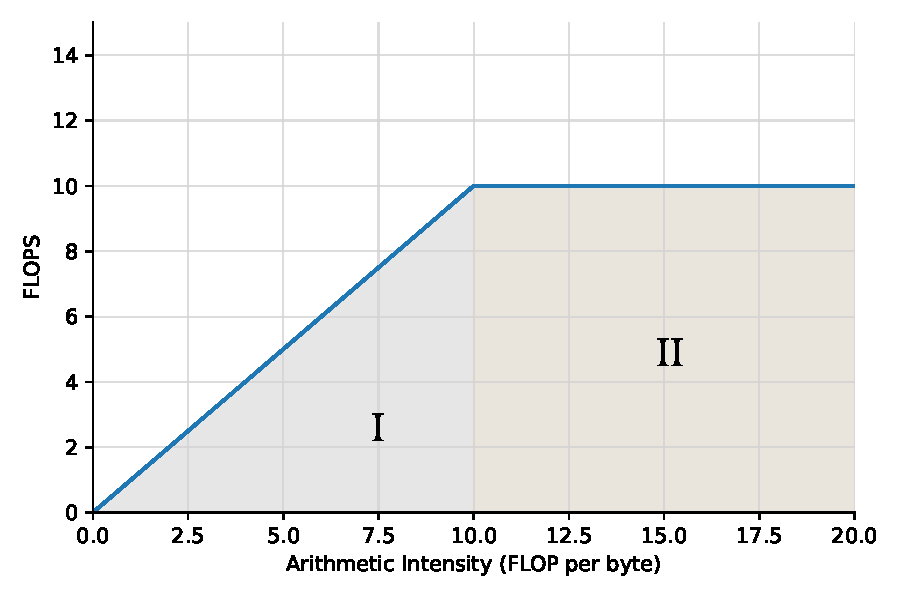
\includegraphics[width=1.0\linewidth]{figures/roofline.pdf}
  \caption{Roofline 模型中可达性能 $ P $ 关于计算强度 $ I $ 的关系图}
  % \note{注:图中的 I 区域代表由于内存带宽限制了可达性能的访存瓶颈(Memory bound)区,而 II 区域代表由于运算器速率限制了可达性能的计算瓶颈(Compute bound)区。这里假设计算系统参数 $\pi$ = 10 FLOPS,$\beta$ = 1 字节。}
  \label{fig:roofline_graph}
\end{figure}

总的来看,基于分析的模型的优秀表现依赖于对待建模架构的深入理解,以及对待建模架构的较详细的微架构基准测试。这赋予了这类模型相对精确的精度,然而也让此类模型的通用性下降。故而,本文提出的方法选择使用基于学习的模型。

% Analytical-based models can be roughly divided into \textit{architecture simulators} and \textit{simple analytical models}. \textit{Architecture simulators} are hand-crafted simulators that are usually cycle accurate for the architecture components that are related to performance. For example, NaviSim \cite{10.1145/3559009.3569666} is a simulator for AMD RDNA architecture, giving predictions on compute kernel execution time by writing simulation procedures for wavefront dispatching, RDNA instruction issuing, decoding and execution. GPGPU-Sim \cite{9138922, 4919648} is a simulator for CUDA / OpenCL workloads that runs on NVIDIA GPUs. \textit{Simple analytical models}, on the other hand, tend to use simple abstractions that capture the common aspects for the architecture family they model. Popular choices of these models includes the roofline model \cite{10.1145/1498765.1498785, KONSTANTINIDIS201737} and the pipeline model \cite{LEMEIRE202332, 10289219, 10.1145/3524059.3532396}. To summarize, analytical-based models in general require a in-depth understanding of the architecture they model as well as extensive micro-benchmarks related to characteristics they capture.

\subsection{基于学习的模型}

% Learning-based models alleviate the need for detailed architecture inspection by using machine learning, and they are much easier to be ported to new architectures given measurements on new architectures. Several works estimate basic block throughput on CPU using either hierarchical LSTM \cite{pmlr-v97-mendis19a} or Graph Neural Network (GNN) \cite{9975403} capturing from in-the-wild application profiles \cite{pmlr-v97-mendis19a, 9042166}. \citet{10.1145/3575693.3575737} modeled the tensor program tuning problem as a Natural Language Processing (NLP) regression task.

相比于基于分析的模型,基于学习的模型通过机器学习的办法,从目标架构的测量数据出发来以较为统一和自动的方式进行架构性能的建模。例如,一些工作采用层次化 LSTM 网络或 GNN 网络 \cite{pmlr-v97-mendis19a, 9975403}来预测给定中央处理器上的基本块吞吐率。如 \citet{10.1145/3575693.3575737} 的工作则将张量程序调优的问题建模为一个采用自然语言处理领域技术的回归任务。

一个比较典型的例子是 Ithemal \cite{pmlr-v97-mendis19a}。如图 \ref{fig:ithemal_overall} 所示,该工作利用了一个 Hierarchical LSTM 网络来预测一个基本块的吞吐率。每条基本块中的指令会经历一个正则化过程来将源操作数、目标操作数等处理成为统一的形式,并送入指令层 LSTM 中。随后,每个指令的隐藏层表示会被送入预测层,并在输入整个序列后输出对该基本块在给定平台上吞吐率的预测。

\begin{figure}[ht]
  \centering
  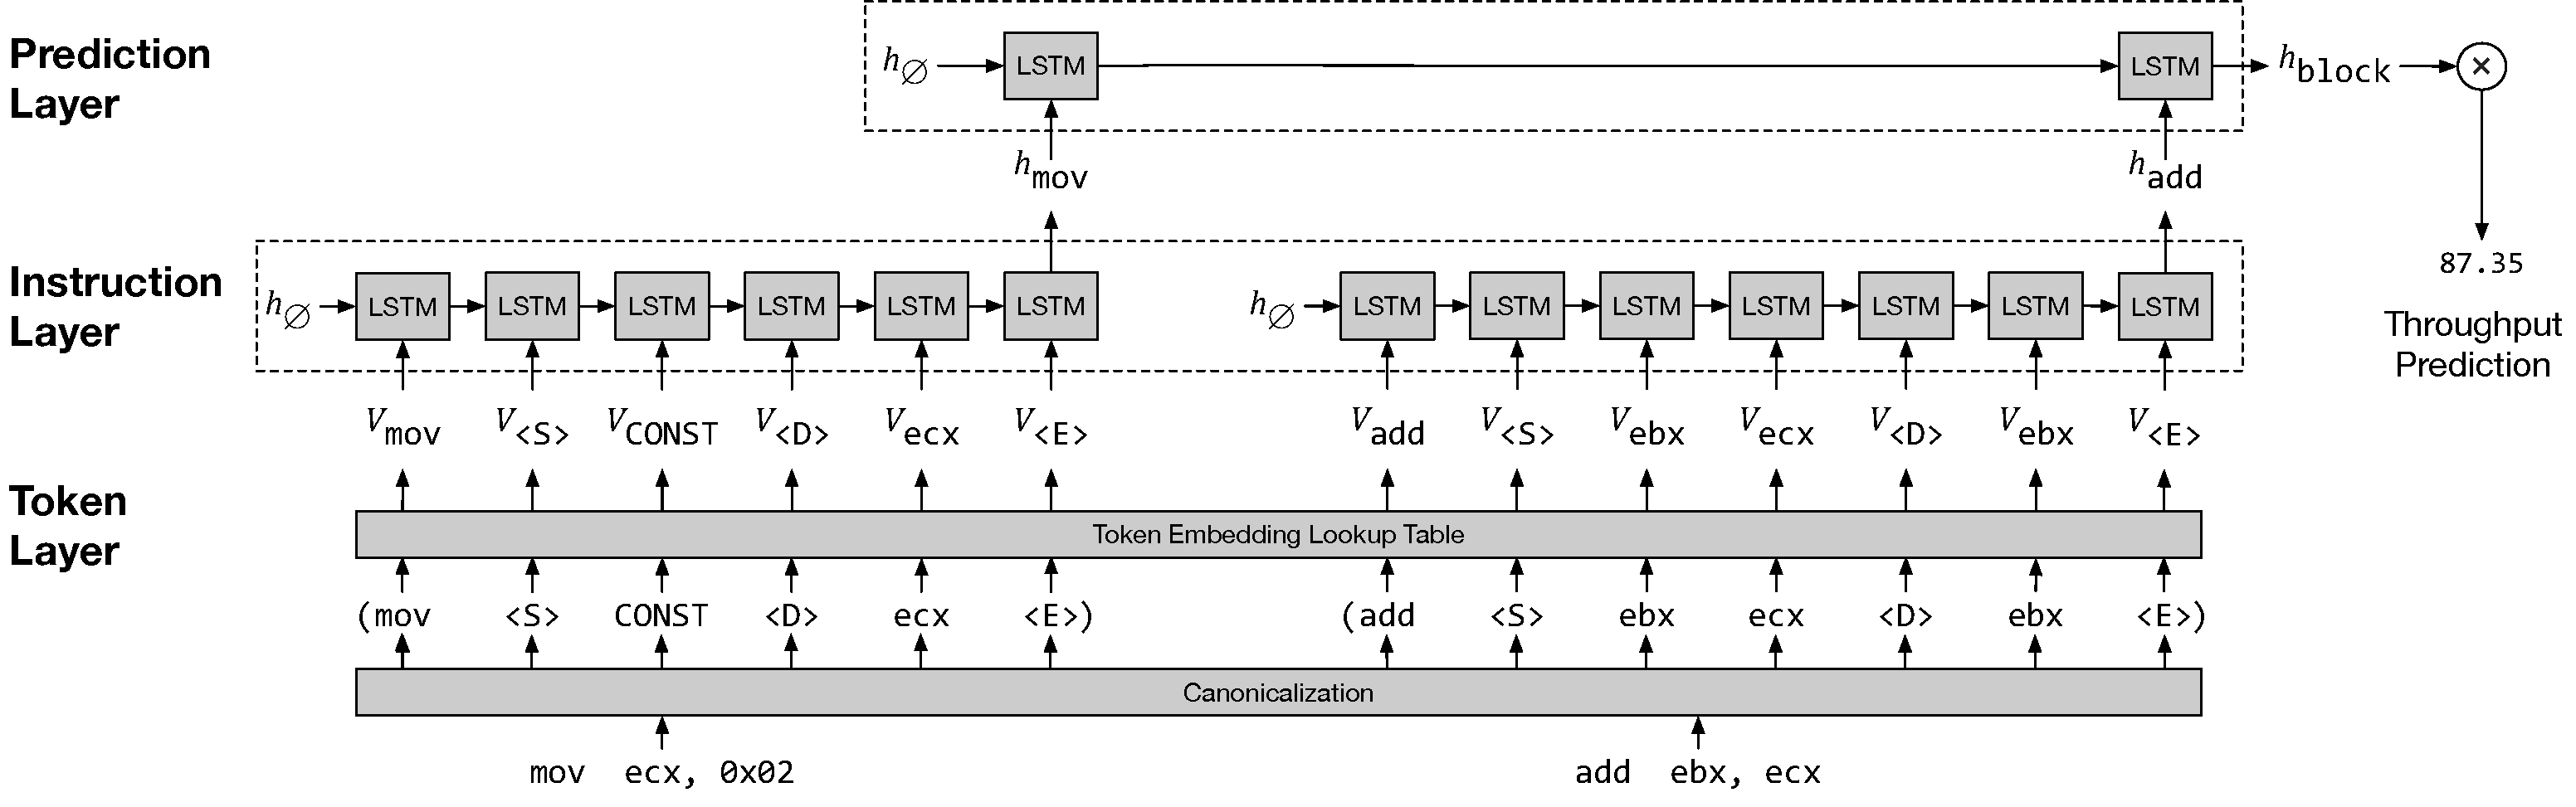
\includegraphics[width=\textwidth]{figures/diag_fullsystem.pdf}
  \vspace{-20pt}
  \caption{Ithemal 网络结构\cite{pmlr-v97-mendis19a}}
  \label{fig:ithemal_overall}
\end{figure}

对于基于学习的模型来说,一个全面而有代表性的训练数据集是模型质量的重要组成部分。Ithemal 的数据集来源于有代表性的用户和系统软件的二进制程序文件,并利用 Dynamorio \cite{10.1145/2365864.2151043} 来导出基本块数据。

% A portion of performance models focus on modeling graphics system performance. \citet{10.1145/3126557} have built a predictive model using random forests for GPU graphics workloads targeting on Intel Skylake integrated graphics, using the internal cycle-accurate simulator as target for alignment. \citet{10.1145/3307650.3322221} proposes Emarald, a SoC simulator built upon GPGPU-Sim \cite{4919648} for graphics and GPGPU system modeling. \citet{8167756} builds GLTraceSim, a framework for generating and replaying CPU and GPU memory traces under graphics workload.

% Our work proposes a learning-based model, as GPU tends to have big architecture differences across vendors and generations. To our knowledge, there are currently no publicly available cross-vendor GPU performance models that focus on shader performance modeling and operate in a black-box fashion, and this work aims to bridge this gap.

本文提出的着色器程序性能预测模型属于基于学习的模型,因为 GPU 架构在不同厂商和产品线间通常差异较大,而基于学习的模型会较易迁移。据作者所知,目前尚不存在面向着色器程序、适用于不同厂商的黑盒性能模型,而本文提出的方法将致力于填补这一空白。类似 Ithemal,本文也收集了自己的性能数据集,以服务后续的性能预测模型的学习。

\subsection{图形系统建模}

% TODO: expand each of the following into a paragraph

一部分性能模型专注于图形系统性能的建模。本节将简要总结这些模型和提出这些模型的工作。

针对 Intel Skylake GT3 显示核心,\citet{10.1145/3126557} 构建了一个预测模型来预测给定图形负载设定下每帧绘制完成所需的的时钟周期数(Cycle Per Frame,CPF)。该预测模型采用随机森林来回归利用截帧工具截取的、来自不同游戏的 Direct3D 视角下的一帧,并且其输入是软光栅器渲染该帧时的一些绘制流水线统计数据。该方法本质上是为加速厂商内部使用的硅前性能验证工具服务的,因为其预测输出的回归目标是 Intel 内部使用的专有硅前仿真软件 GPUSim 输出的该帧时钟周期数值,且利用随机森林和软光栅器的方案相较于该时钟精确的 GPUSim 软件来说可以达到平均 327 倍的加速。

\citet{8167756} 提出了 GLTraceSim,一个用于分析 GPU 平台下 GPU 和 CPU 内存系统通信的框架。该框架主要包括截帧、生成内存追踪信息、重放内存追踪信息和分析四个步骤。和 \citet{10.1145/3126557} 的工作类似,该工作也是通过软光栅器来提取相应的传输特征,并且送入相关的细粒度模拟器进行模拟的。图 \ref{fig:gltracesim} 给出了GLTraceSim 中内存访问和 CPU/GPU 同步模拟的大致流程。可以看到,相比于\citet{10.1145/3126557}的工作,GLTraceSim 更详细的抽出了软光栅器 LLVMPipe 中可能与 CPU/GPU 内存访问和同步的相关信息,并且在一个内存系统模拟器上重放来评估给定架构下内存系统的工作效率。

\begin{figure}
    \centering
    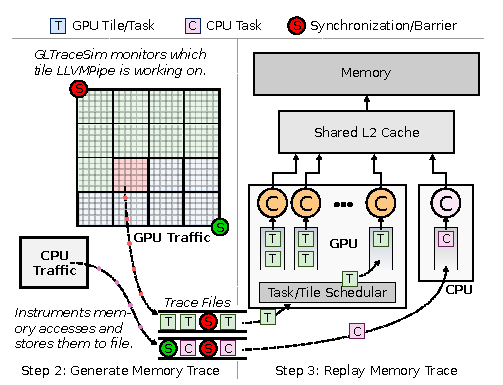
\includegraphics{figures/GLTraceSim.pdf}
    \caption{GLTraceSim 中内存访问和 CPU/GPU 同步模拟流程图\cite{8167756}}
    \label{fig:gltracesim}
\end{figure}

% https://zhuanlan.zhihu.com/p/615066252 - replacement for \textcircled

不过,以上两类工作都只是对 GPU 绘制过程中的部分模块进行了仿真,并提出一些性能特征因子以供下游预测或模拟使用。\citet{10.1145/3307650.3322221} 则更进一步,提出了全系统模拟的 Emarald,一个基于GPGPU-Sim \cite{4919648} 的、可以建模整个 SoC 的内存和计算行为的模拟器。该模拟器可以支持 OpenGL 和 OpenGL ES 着色器的模拟,同时可以配合 gem5 一起进行 Android 全系统模拟。

如图 \ref{fig:emerald_gpu_arch} 所示,Emerald 仿真中的 GPU 包括一个共享的、支持原子操作的 L2 缓存和一系列 SIMT Cluster,其中每个 SIMT Cluster 中的结构如图 \ref{fig:emerald_units}(a) 所示。在每个 SIMT Cluster 中,包括 \ding{172} 中的 SIMT 核心以及 \ding{173} 到 \ding{179} 表示的固定管线单元。渲染管线的顶点着色阶段会在 \ding{172} 中的 SIMT 核心中运行顶点着色器,并由 SIMT 核心将生成后的顶点位置信息送到顶点处理和运算单元 VPO 中。

VPO 的结构如图 \ref{fig:emerald_units}(b) 所示,其会将变换后的图元按屏幕空间的特定顺序分配给不同的 SIMT Cluster。为了实现这个目的,VPO 会将送入的顶点束(vertex warp)进行顶点对应的图元的包围盒计算,并给出其在每个 SIMT Cluster 中是否存在的掩码,之后通过互联网络进行重排序,以让每个 SIMT Cluster 的光栅器最后处理本 SIMT Cluster 负责的屏幕空间区域的图元的光栅化操作。

\begin{figure}
    \centering
    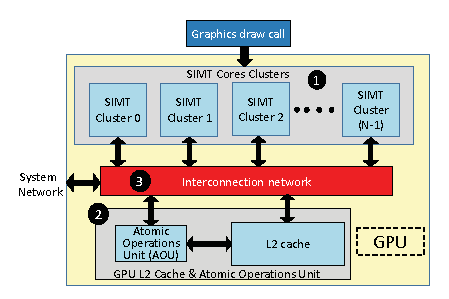
\includegraphics{figures/emerald_gpu_arch.pdf}
    \caption{Emerald 中仿真的 GPU 架构示意图\cite{10.1145/3307650.3322221}}
    \label{fig:emerald_gpu_arch}
\end{figure}

\begin{figure}
    \centering
    \begin{minipage}[b]{\textwidth}
        \begin{subfigure}[b]{0.48\textwidth}
            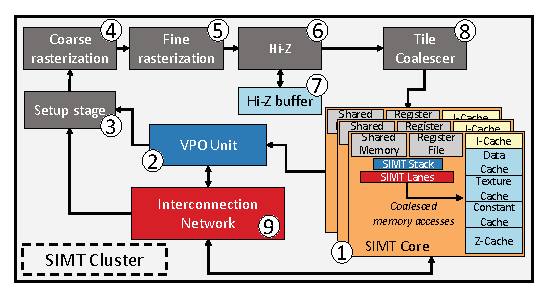
\includegraphics[width=\textwidth, trim=5 0 0 0, clip]{figures/emerald_simt_cluster.pdf}
            \caption{Emerald 中仿真的 SIMT Cluster 示意图}
            \label{fig:sub_simt}
        \end{subfigure}
        % \hfill % Adds horizontal space between the subfigures
        \begin{subfigure}[b]{0.48\textwidth}
            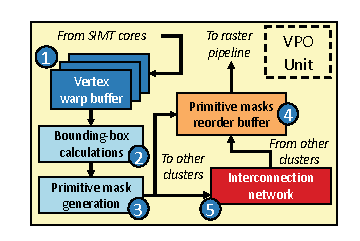
\includegraphics[width=\textwidth, trim=0 5 0 0]{figures/emerald_vpo_unit.pdf}
            \caption{Emerald 中仿真的 VPO 单元示意图}
            \label{fig:sub_vpo}
        \end{subfigure}
    \end{minipage}
    
    %\vspace{1em} % Adds vertical space between the rows of subfigures

    % TODO: add reference
    \caption{Emerald 中仿真的 GPU 架构中的细粒度单元示意图\cite{10.1145/3307650.3322221}}
    \label{fig:emerald_units}
\end{figure}

% TODO: crop the picture and explain; SC is shader core, inside which it does the detailed emulation, so no magic here



% TODO: summarize

总的来说,这些工作多着眼于和给定的图形处理器架构精确对齐,且大多需要对待建模架构的较深入理解,或者一些厂商内部模型的指导。故而,其对于图形程序员的帮助有限,且测试和使用均需要逐平台进行,因而也受到跨平台性能调优面临的平台碎片化的困难的影响。正因如此,本研究选择从数据驱动驱动的方法出发,通过神经网络方法来建模着色器程序的性能。
